\documentclass[12pt]{article}
    \usepackage[margin=1in]{geometry}
    \usepackage{amsmath, amssymb}
    \usepackage{graphicx}
    \usepackage{booktabs}
    \usepackage{hyperref}
    \usepackage{float}
    \usepackage{caption}
    \usepackage{subcaption}
    \usepackage{xcolor}

    \title{CSc 8830 --- Module 9 Assignment\\\\Uncalibrated Stereo: Distance Estimation}
    \author{Achindra Baruah}
    \date{\today}

    \begin{document}
    \maketitle

    % ──────────────────────────────────────────────────────────
    \section{Introduction}

    This report presents the results of using an \textbf{uncalibrated stereo camera setup} to observe objects in a classroom and estimate the distance to a selected object of interest. The stereo pair was captured with an iPhone 16 Pro Max (24\,mm $f$/1.78 main camera) at two positions separated by a known baseline.

    The pipeline computes the \textbf{Fundamental Matrix} ($\mathbf{F}$), the \textbf{Essential Matrix} ($\mathbf{E}$), and decomposes $\mathbf{E}$ into the \textbf{Rotation Matrix} ($\mathbf{R}$) and translation vector ($\mathbf{t}$). Feature-point triangulation is then used to estimate the distance to the selected object.

    % ──────────────────────────────────────────────────────────
    \section{Setup}

    \begin{table}[H]
    \centering
    \begin{tabular}{ll}
    \toprule
    \textbf{Parameter} & \textbf{Value} \\
    \midrule
    Camera & iPhone 16 Pro Max --- 24\,mm $f$/1.78 \\
    Resolution & 5712 $\times$ 4284 (24 MP) \\
    Baseline & 1.50\,m \\
    Processing resolution & Working scale \\
    Focal length (full) & 3808\,px \\
    Focal length (scaled) & 1066.7\,px \\
    \bottomrule
    \end{tabular}
    \caption{Camera and setup parameters.}
    \end{table}

    \begin{figure}[H]
    \centering
    \includegraphics[width=\textwidth]{stereo_pair.png}
    \caption{Stereo pair: left image and right image captured from two positions.}
    \end{figure}

    % ──────────────────────────────────────────────────────────
    \section{Intrinsic Matrix}

    Since we know the camera is an iPhone 16 Pro Max with a 24\,mm equivalent focal length, the horizontal field of view is:
    \[
    \text{HFoV} = 2 \cdot \arctan\!\left(\frac{36}{2 \cdot 24}\right) \approx 73.7^\circ
    \]
    The pixel focal length at the full resolution $W = 5712$ is:
    \[
    f_{px} = \frac{W}{2 \cdot \tan(\text{HFoV}/2)} = \frac{5712}{2 \cdot \tan(36.85^\circ)} \approx 3808 \text{ px}
    \]
    The intrinsic matrix (at working resolution) is:
    \[
    \mathbf{K} = \begin{bmatrix}
 1.07e+03 &  0.00e+00 &  8.00e+02 \\
 0.00e+00 &  1.07e+03 &  6.00e+02 \\
 0.00e+00 &  0.00e+00 &  1.00e+00
\end{bmatrix}
    \]

    % ──────────────────────────────────────────────────────────
    \section{Feature Matching}

    SIFT features were detected in both images and matched using brute-force matching with Lowe's ratio test (threshold 0.65). A total of \textbf{484} good matches were found, of which \textbf{265} were kept as inliers after RANSAC.

    \begin{figure}[H]
    \centering
    \includegraphics[width=\textwidth]{feature_matches.png}
    \caption{SIFT feature matches between left and right images (top 100 shown).}
    \end{figure}

    % ──────────────────────────────────────────────────────────
    \section{Fundamental Matrix ($\mathbf{F}$)}

    The Fundamental Matrix encodes the epipolar geometry between the two views. For corresponding points $\mathbf{x}$ and $\mathbf{x'}$ in the left and right images:
    \[
    \mathbf{x'}^\top \mathbf{F} \, \mathbf{x} = 0
    \]
    $\mathbf{F}$ was computed using the 8-point algorithm within a RANSAC framework:
    \[
    \mathbf{F} = \begin{bmatrix}
 2.56396728e-07 & -4.05445638e-06 &  1.92571339e-03 \\
 3.38093533e-06 &  2.93144287e-07 & -5.33044117e-03 \\
-2.13060162e-03 &  3.94302750e-03 &  1.00000000e+00
\end{bmatrix}
    \]
    \textbf{Verification:} The mean epipolar error $|\mathbf{x'}^\top \mathbf{F} \mathbf{x}|$ across all inliers is $\mathbf{0.000985}$, confirming the accuracy of~$\mathbf{F}$.

    \begin{figure}[H]
    \centering
    \includegraphics[width=\textwidth]{epipolar_lines.png}
    \caption{Epipolar lines drawn on both images. Each colour represents a corresponding point pair. The lines pass through (or very near) the corresponding points, verifying~$\mathbf{F}$.}
    \end{figure}

    % ──────────────────────────────────────────────────────────
    \section{Essential Matrix ($\mathbf{E}$)}

    The Essential Matrix relates the normalised image coordinates and encodes the relative pose (rotation and translation) between the two cameras:
    \[
    \mathbf{E} = \mathbf{K}^\top \mathbf{F} \, \mathbf{K}
    \]
    After enforcing the rank-2 constraint via SVD (setting $\sigma_3 = 0$ and equalising $\sigma_1 = \sigma_2$):
    \[
    \mathbf{E} = \begin{bmatrix}
 2.6911e-01 & -4.5868e+00 & -3.0585e-01 \\
 3.8690e+00 &  3.6203e-01 & -2.6275e+00 \\
 1.1543e-01 &  9.2972e-01 & -5.3864e-02
\end{bmatrix}
    \]
    \textbf{Singular values:} $\sigma_1 = 4.6952$, $\sigma_2 = 4.6952$, $\sigma_3 = 0.0000$.

    For a valid Essential matrix, we require $\sigma_1 \approx \sigma_2$ and $\sigma_3 \approx 0$, which is satisfied.

    % ──────────────────────────────────────────────────────────
    \section{Rotation Matrix ($\mathbf{R}$) and Translation ($\mathbf{t}$)}

    The Essential matrix is decomposed into the relative camera rotation and translation:
    \[
    \mathbf{E} = [\mathbf{t}]_\times \mathbf{R}
    \]
    Using SVD decomposition with the chirality check (selecting the solution where triangulated points are in front of both cameras):
    \[
    \mathbf{R} = \begin{bmatrix}
 9.183953e-01 &  7.972447e-02 & -3.875489e-01 \\
-7.546602e-02 &  9.968036e-01 &  2.622121e-02 \\
 3.884006e-01 &  5.165336e-03 &  9.214761e-01
\end{bmatrix}
    \]
    \[
    \mathbf{t} = \begin{bmatrix} -0.195225 \\  0.042811 \\ -0.979824 \end{bmatrix}
    \]

    \textbf{Verification:}
    \begin{itemize}
    \item $\det(\mathbf{R}) = 1.000000$ (should be $+1$ for a proper rotation)
    \item $\|\mathbf{R}^\top\mathbf{R} - \mathbf{I}\| = 6.70e-16$ (should be $\approx 0$)
    \item Rotation angle: $23.32^\circ$
    \item $\|\mathbf{t}\| = 1$ (unit norm from \texttt{recoverPose}; scale set by baseline)
    \end{itemize}

    % ──────────────────────────────────────────────────────────
    \section{Distance Estimation}

    \subsection{Method}
    The distance to the selected object is estimated using the stereo disparity of matched feature points. For corresponding points $(u_L, v)$ and $(u_R, v)$ in the left and right images, the disparity is $d = u_L - u_R$ and the depth is:
    \[
    Z = \frac{f \cdot b}{d}
    \]
    where $f = 1066.7$\,px is the focal length and $b = 1.50$\,m is the baseline.

    SIFT feature correspondences (RANSAC inliers) falling within or near the object's bounding box are used, and the \textbf{median disparity} of these matches gives a robust depth estimate.

    \subsection{Object Selection}
    The object of interest --- \textbf{table} --- was detected using YOLOv8x. Feature matches within the bounding box region are used to compute the median disparity.

    \begin{figure}[H]
    \centering
    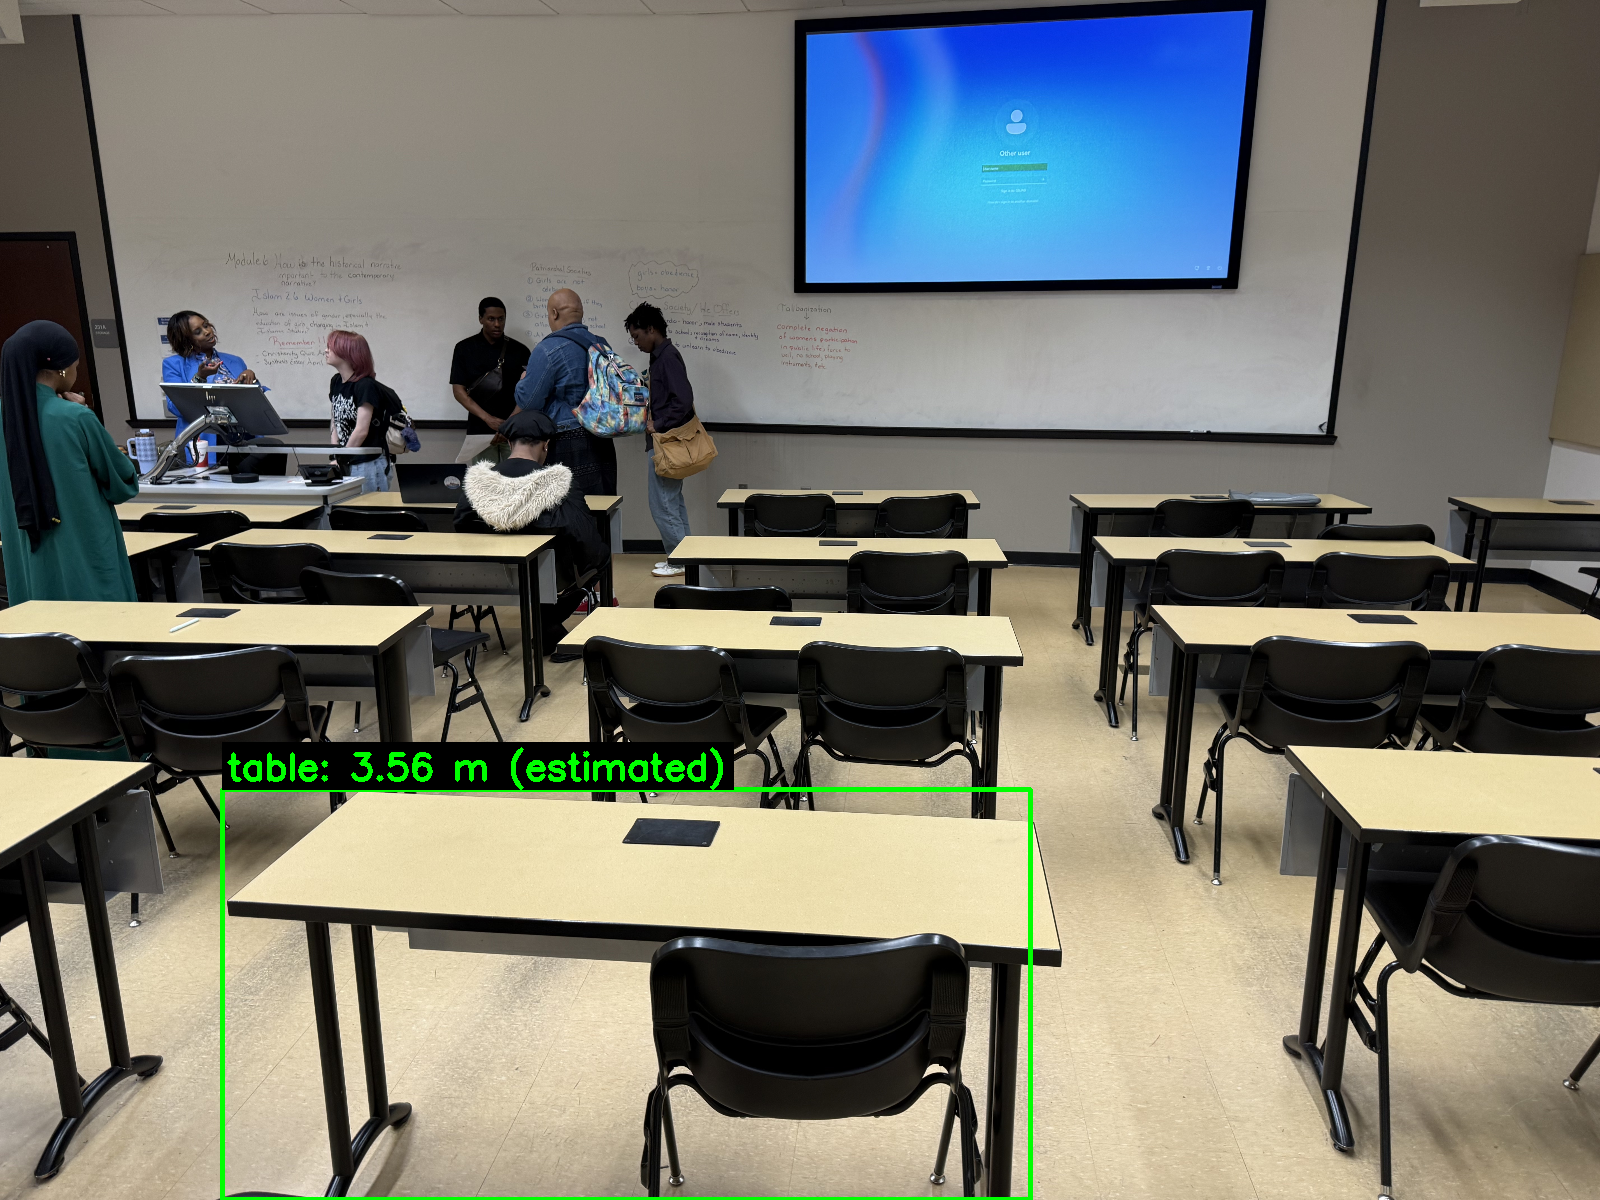
\includegraphics[width=0.8\textwidth]{annotated_object.png}
    \caption{Selected object (\textbf{table}) with estimated distance annotation.}
    \end{figure}

    \subsection{Result}
    \begin{table}[H]
    \centering
    \begin{tabular}{ll}
    \toprule
    \textbf{Quantity} & \textbf{Value} \\
    \midrule
    Selected object & table \\
    Matched points used & 47 \\
    Median disparity & 450.0\,px \\
    Focal length & 1066.7\,px \\
    Baseline & 1.50\,m \\
    \textbf{Estimated distance} & \textbf{3.56\,m} \\
\bottomrule
\end{tabular}
\caption{Distance estimation results.}
\end{table}



% ──────────────────────────────────────────────────────────
\section{Summary Figure}

\begin{figure}[H]
\centering
\includegraphics[width=\textwidth]{summary.png}
\caption{Complete pipeline summary: (a) stereo pair, (b) feature matches, (c) epipolar verification, (d) object annotation with distance estimate.}
\end{figure}

% ──────────────────────────────────────────────────────────
\section{Conclusion}

Using an uncalibrated stereo setup with an iPhone 16 Pro Max, we successfully:
\begin{enumerate}
\item Computed the Fundamental Matrix $\mathbf{F}$ from SIFT correspondences (verified by epipolar constraint).
\item Derived the Essential Matrix $\mathbf{E} = \mathbf{K}^\top \mathbf{F} \mathbf{K}$ using known iPhone intrinsics.
\item Decomposed $\mathbf{E}$ into the camera rotation $\mathbf{R}$ ($23.32^\circ$) and unit translation $\mathbf{t}$.
\item Triangulated scene points and estimated the distance to the selected object (\textbf{table}) as \textbf{3.56\,m}.
\end{enumerate}

\end{document}
